\begin{enumerate}[label=\textbf{\alph*)}]
      \item{
                  \hfill

                  El diagrama se puede apreciar en la \ut{fig. \ref{fig:ccst}}
            }

      \vspace{\baselineskip}

      \item  Como se trata de un proceso reversible  sabemos que:
            \[ \dbar Q =TdS \]
            El proceso de $A$ a $B$ se trata de un proceso isotermico, por lo que si integramos la expresión anterior tenemos:
            \[ \int \dbar Q =T_{c}\int dS \]
            \[ \Rightarrow \int _{v_A} ^{v_B} \dbar Q = T_{c} \Delta S\]
            \[nRT_c \ln \left( \frac{v_B}{v_A}\right) = T_{c}\Delta S = Q_{entrada}\]
            En el proceso de $B$ a $C$ al tratarse de un proceso adiabático, no hay intercambio de calor $\Rightarrow Q=0$\\

            En  el proceso de $C$ a $D$ tenemos un proceso isotermico, por lo que analogamente al proceso de $A$ a $B$ tenemos:

            \[ \int \dbar Q =T_{f}\int dS \]
            \[ \Rightarrow \int _{v_C} ^{v_D} \dbar Q = T_{f} \Delta S\]
            \[nRT_f \ln \left( \frac{v_D}{v_C}\right) = T_{f}\Delta S = Q_{salida}\]

            Como se trata de un calor de salida
            \[Q_{salida}=-nRT_c \ln \left( \frac{v_D}{v_C}\right)\]


            Ahora bien si  se trata de un gas ideal y el proceso se realiza a presión constante tenemos que:
            \[ \frac{v_1}{T_1}=\frac{v_2}{T_2}\]
            \[\Rightarrow \frac{T_2}{T_1}=\frac{v_2}{v_1}\]

            Entonces tenemos que:
            \[ \frac{v_B}{v_A}=\frac{Tf}{Tc}=\frac{v_D}{v_c}\]

            Tenemos que la eficiencia esta dada por:
            \[ \eta = \frac{Q_{entrada}+ Q_{salida}}{Q_{entrada}}\]

            \[\Rightarrow  \eta = \frac{nRT_c \ln \left( \frac{v_B}{v_A}\right)-nRT_f \ln \left( \frac{v_D}{v_C}\right)}{nRT_c \ln \left( \frac{v_B}{v_A}\right)}\]
            \[\Rightarrow  \eta = \frac{nRT_c \ln \left( \frac{v_B}{v_A}\right)-nRT_f \ln \left( \frac{v_B}{v_A}\right)}{nRT_c \ln \left( \frac{v_B}{v_A}\right)}\]
            \[\eta =\frac{T_c-T_f}{T_c}\]

            \begin{figure}[H]
                  \centering
                  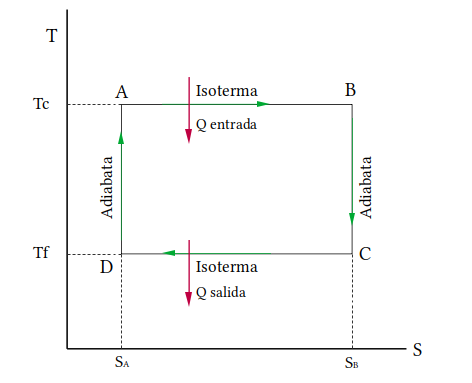
\includegraphics[width=0.65\textwidth]{T-S.png}
                  \caption{Diagrama de un ciclo de Carnot para un gas ideal
                        en el plano \ut{T - S}}
                  \label{fig:ccst}
            \end{figure}



\end{enumerate}
